\subsection{Systeemmodellen}
\subsubsection{Datamodel}
Na een brainstormsessie met alle groepsleden is het volgende model bedacht om de verschillende entiteiten in te delen.
\begin{figure}[htp]
\begin{center}
	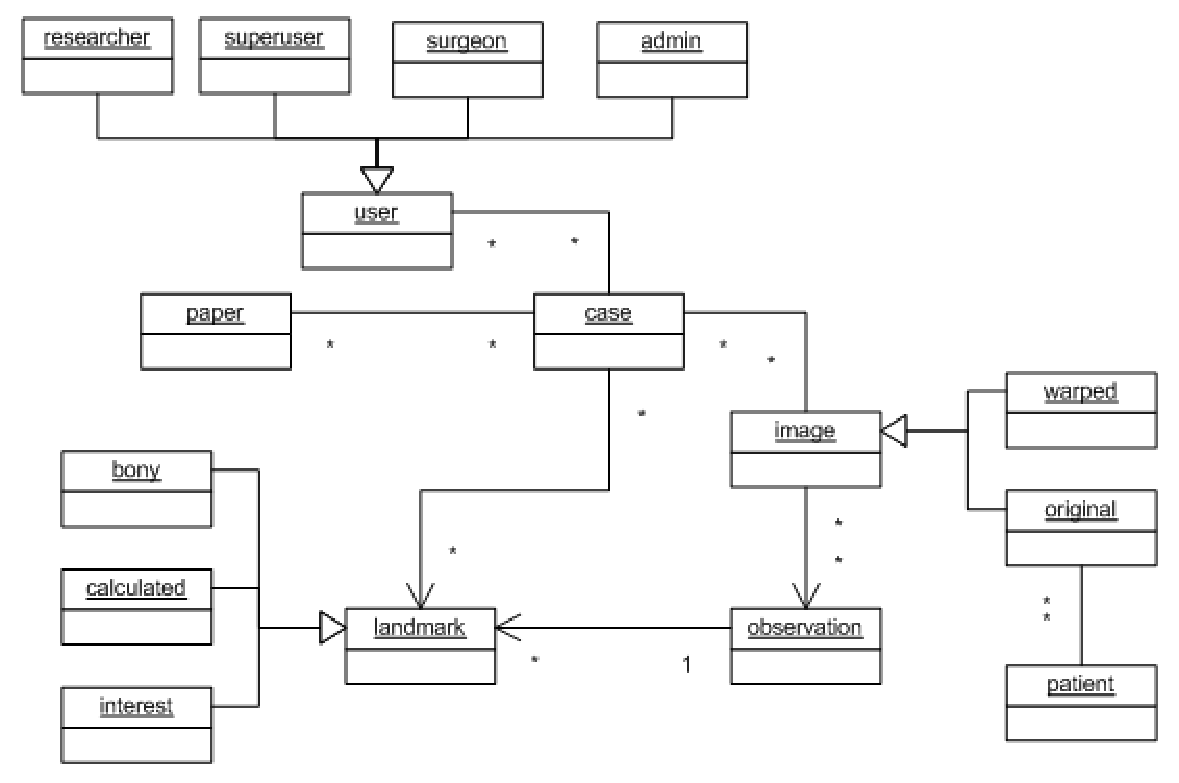
\includegraphics[scale=0.65]{brainstorm_klassediagram}
\caption{Datamodel}
\label{default}
\end{center}
\end{figure}


\section{Scenario's}

%%%%%%%%%%%%%%%%%%%%%%%%%%%%%%%%%%%%%%%%%%%%%%%%%%%%%%%%%%%%%%%%%%%%%%%%%%%%%%%%%%%%%%%%%%%
%% Algemeen
In deze paragraaf beschrijven we use cases van gebruikers die het systeem voor verschillende doeleinden willen inzetten.

\begin{enumerate}

\item   Naam: Add new project  \\
	Actor:
	\begin{itemize}
		\item Anton: Gebruiker met onderzoeker account
	\end{itemize}
	Flow of events
	\begin{enumerate}
		\item Anton heeft van Dr. Kleinrensink een nieuw project gekregen en wil dit in het systeem zetten.
		\item Hij klikt op de 'voeg nieuw project toe' knop in het hoofdscherm.
		\item In het volgende scherm vult hij de naam en beschrijving van het project toe.
		\item Hij komt nu in het scherm van het zojuist gemaakte project en kan nu meteen foto's en/of metingen toevoegen.
	\end{enumerate}
\end{enumerate}

\item   Naam: Add Image \\
	Actor:
	\begin{itemize}
		\item Anton: Gebruiker met onderzoeker account
	\end{itemize}
	Flow of events
	\begin{enumerate}
        \item Anton wil een foto toevoegen aan een bestaand project
				\item Hij selecteert eerst het project kiest ervoor om een nieuwe foto toe te voegen
				\item Vervolgens voegt Anton de aanvullende gegevens over de foto toe en de foto zelf en klikt op 'Toevoegen' 
				\item Het resultaat (toegevoegde foto aan relevant project) wordt getoond.
    \end{enumerate}


\item  Naam: View Images  \\
	Actor:
	\begin{itemize}
		\item Anton: Gebruiker met onderzoeker account
		\item Dr. Kleinrensink: Gebruiker met chirurg account
	\end{itemize}
	Flow of events
	\begin{enumerate}
		\item De actor wil een aantal plaatjes bekijken van een project.
		\item Hij selecteert het project en klikt op de aanwezige thumbnails.
		\item Nu krijgt hij alle images te zien voor dat project met aan de rechterkant een sidebar.
		\item In deze sidebar kan hij aangeven welke plaatjes hij wil zien en met welke metingen. Ook kan hij de doorzichtigheid van de plaatjes aangeven om verschillende plaatjes tegelijk te belijken.
	\end{enumerate}
\end{enumerate}

\item   Naam: Remove Images \\
	Actor:
	\begin{itemize}
		\item Anton: Gebruiker met onderzoeker account
	\end{itemize}
	Flow of events
	\begin{enumerate}
		\item Er is een foute foto ingevoerd die niet in dat project hoort.
		\item Hij selecteert het project waar de foto in zit en klikt op de foute foto.
		\item In de detailed view van de foto klikt hij op 'verwijder foto'.
		\item Het systeem verwijderd nu de foto en de geassocieerde data.
	\end{enumerate}
\end{enumerate}

\item   Naam: Add Measurement from existing type  \\
	Actor:
	\begin{itemize}
		\item Anton: Gebruiker met onderzoeker account
	\end{itemize}
	Flow of events
	\begin{enumerate}
		\item Anton wil een nieuwe meting of landmark toevoegen aan een foto.
		\item Hij selecteert het project en klikt erop.
		\item Hierna klikt hij op de foto waarvan hij de meting of landmark wil toevoegen of voegt hij een nieuwe foto toe.
		\item Hij klikt vervolgens in de foto om een meting of landmarkt toe te voegen.
		\item Hierna kiest hij het type meting en bevestigd.
		\item Als de meting of landmark goed staat bevestigd hij de positie. Als het nog niet goedstaat kan de positie nog gewijzigd worden.
	\end{enumerate}
\end{enumerate}

\item   Naam: Add new Measurement type  \\
	Actor:
	\begin{itemize}
		\item Anton: Gebruiker met onderzoeker account
	\end{itemize}
	Flow of events
	\begin{enumerate}
		\item Anton wil een nieuw type meting toevoegen aan een project.
		\item Hij opent het project waar de meting bijhoort.
		\item Hij voegt de meting toe door op het plusje te klikken in de lijst met metingen typen.
		\item Hierna voert hij het type meting in (punt, lijn, oppervlakte).
		\item Het metingtype staat nu in de lijst met mogelijke metingen voor het project.
	\end{enumerate}
\end{enumerate}

\item   Naam: Edit existing measurement  \\
	Actor:
	\begin{itemize}
		\item Anton: Gebruiker met onderzoeker account
	\end{itemize}
	Flow of events
	\begin{enumerate}
		\item Anton wil een meting bewerken die hij al had opgeslagen.
		\item Hij klikt het juiste project aan en selecteerd de foto waarop de meting is gedaan.
		\item Hij selecteert nu de te wijzigen meting en herpositioneert deze of past de waarde ervan aan.
		\item Hij bevestigd de nieuwe waarde en slaat zijn meting op.
	\end{enumerate}
\end{enumerate}

\item   Naam: Remove measurement  \\
	Actor:
	\begin{itemize}
		\item Anton: Gebruiker met onderzoeker account
	\end{itemize}
	Flow of events
	\begin{enumerate}
		\item Anton wil een meting verwijderen.
		\item Hij klikt het juiste project aan en selecteerd de foto waarop de meting is gedaan.
		\item Hij selecteert nu de te verwijderen meting en verwijdert deze.
		\item De meting zelf is nu verwijderd maar het type meting blijft bestaan in het project
	\end{enumerate}
\end{enumerate}

\item   Naam: Remove measurement type  \\
	Actor:
	\begin{itemize}
		\item Anton: Gebruiker met onderzoeker account
	\end{itemize}
	Flow of events
	\begin{enumerate}
		\item Anton wil een type meting verwijderen.
		\item Hij klikt het juiste project aan.
		\item Hij selecteert nu het te verwijderen metingtype en verwijdert deze.
		\item Het type meting en alle metingen die eraan verbonden zijn worden verwijderd.
	\end{enumerate}
\end{enumerate}

\item   Naam: View measurements \\
	Actor:
	\begin{itemize}
		\item Anton: Gebruiker met onderzoeker account
		\item Dr. Kleinrensink: Gebruiker met chirurg account
	\end{itemize}
	Flow of events
	\begin{enumerate}
		\item De actor wil de metingen van een project zien.
		\item Hij selecteert het project en klikt op de foto('s) waarvan hij de metingen wil zien.
		\item In de sidebar kan hij vervolgens aangeven welke metingen hij wil zien en op welke manier ze geprojecteerd moeten worden.
	\end{enumerate}
\end{enumerate}

\item   Naam: Add Related Papers (lokaal, online (pubmed), powerpoints) \\
	Actor:
	\begin{itemize}
		\item Anton: Gebruiker met onderzoeker account
		\item Dr. Kleinrensink: Gebruiker met chirurg account
	\end{itemize}
	Flow of events
	\begin{enumerate}
		\item De actor wil gerelateerde papers aan een project toevoegen.
		\item Hij selecteerd het project.
		\item Bij de weergegeven papers klikt hij op paper toevoegen.
		\item Hij kan nu een paper uploaden of een link toevoegen naar een PubMed publicatie.
		\item De paper wordt nu weergegeven in de lijst met gerelateerde papers.
	\end{enumerate}
\end{enumerate}

\item   Naam: View Related Papers (lokaal, online (PubMed), powerpoints)  \\
	Actor:
	\begin{itemize}
		\item Anton: Gebruiker met onderzoeker account
		\item Dr. Kleinrensink: Gebruiker met chirurg account
	\end{itemize}
	Flow of events
	\begin{enumerate}
		\item De actor wil gerelateerde papers van een project bekijken.
		\item Hij selecteerd het project.
		\item De gerelateerde papers worden weergegeven. 
	\end{enumerate}
\end{enumerate}

\item   Naam: Change User Password \\
	Actor:
	\begin{itemize}
		\item Anton: Gebruiker met onderzoeker account
		\item Dr. Kleinrensink: Gebruiker met chirurg account
		\item Xanthos: Gebruiker met beheerder account
	\end{itemize}
	Flow of events
	\begin{enumerate}
		\item De actor wil zijn wachtwoord wijzigen.
		\item Hij logt in op het systeem.
		\item Hij kiest ervoor zijn wachtwoord te veranderen.
		\item Hij voert nu het oude wachtwoord in en tweemaal het nieuwe.
		\item Het wachtwoord is gewijzigd.
	\end{enumerate}
\end{enumerate}

\item   Naam: Add User  \\
	Actor:
	\begin{itemize}
		\item Xanthos: Gebruiker met beheerder account
	\end{itemize}
	Flow of events
	\begin{enumerate}
	  \item De beheerder wil een nieuwe gebruiker toevoegen.
		\item Hij logged in op het beheerders gedeelte.
		\item Hij voert de inlognaam en de toegangsrechten toe.
		\item Het wachtwoord en de inlognaam wordt getoond
	\end{enumerate}
\end{enumerate}

\item   Naam: Edit User  \\
	Actor:
	\begin{itemize}
		\item Xanthos: Gebruiker met beheerder account
	\end{itemize}
	Flow of events
	\begin{enumerate}
	  \item De beheerder wil een gebruikersaccount bewerken.
		\item Hij logged in op het beheerders gedeelte.
		\item Hij selecteert de gebruiker.
		\item Het password kan nu gereset worden, de gebruikersnaam gewijzigd of de toegangsrechten aangepast.
	\end{enumerate}
\end{enumerate}


\item   Naam: Remove User  \\
	Actor:
	\begin{itemize}
		\item Xanthos: Gebruiker met beheerder account
	\end{itemize}
	Flow of events
	\begin{enumerate}
	  \item De beheerder wil een gebruikersaccount verwijderen.
		\item Hij logged in op het beheerders gedeelte.
		\item Hij selecteert de gebruikersaccount.
		\item De gebruikersaccount kan nu verwijderd worden
	\end{enumerate}
\end{enumerate}



